\section{Evaluation}
\label{sec:evaluation}

This section presents our evaluation.
We introduce our experimental setup and benchmark
design.
We then evaluate different placement schemes
by measuring query throughput and
testing their robustness to slight workload mispredictions.


\subsection{Experiment Setup}

We conducted our evaluation on Virtual Computing Lab (VCL), a cloud
platform provided by NC State University.
All servers are equipped with 2-core Intel Xeon CPU and 8GB memory
and connected to a 10 Gbit switch. 
VCL only provides limited storage capacity of local disks or
\emph{instance storage}.
This is also the case for many cloud configurations.
In fact, a majority of EC2 instance types in Amazon Web Services (AWS) do not
have any instance storage.
Instead one must mount a remote volume served by a enterprise-level
storage system.
(AWS calls this \emph{elastic block storage}--EBS.)
We evaluate our approach using both instance storage (local disks) and
remote volumes provided by network file system (NFS),
backed by NetApp 2554 filer with dual controllers.

We evaluate our placement schemes on
high performance computing cluster (HPCC)~\cite{middleton2011hpcc}.
HPCC is an open source
data analytics computer developed by LexisNexis Risk
Solutions for processing big data.
They maintain several clusters with more than 100 nodes, the largest
with more than 500, to provide services to their clients.
Experiments were conducted on a HPCC Roxie cluster.
Roxie is a \emph{data delivery engine} that responds to queries.
It finds the answers to requests in an index that is partitioned and,
if desired, replicated across the nodes.
Roxie is optimized to handle massive amounts of concurrent requests
with low latency.

Data replication and placement that fit workload demands
have direct performance impact on performance.
Roxie clusters partition and distribute data
with two replicas per partition by default.
We modified Roxie to incorporate our data placement schemes.
Our approaches are not specific to Roxie.
They should be able to apply to
Apache Hadoop, HBase, Cassandra, and Ceph, providing benefit when
workloads are not uniformly distributed across
keys, partitions or nodes.


\subsection{Workload Generator and Benchmark Suite}

To evaluate the results learned in our simulation, we developed a
distributed benchmark tool 
that is able to issue a large volume of concurrent queries to
Roxie. 
This benchmark tool adopts the master-slave architecture, where
the the master node generates workload according to a workload profile, and
the slave nodes execute the query requests.
This tool is customizable and supports any number of
workload distributions.
This benchmark suite is written in Python, and designed for testing
query performance at large scale.

In our evaluation, we are interested in how placement schemes
with different levels of partition granularity
respond to different types of workload distribution.
We consider \emph{uniform}, \emph{beta}, \emph{power law}, \emph{normal}, and \emph{gamma} distributions.
The beta distribution is defined on the interval $[0, 1]$ with
two shape parameters, $\alpha$ and $\beta$.
We choose $\alpha=2$ and $\beta=2$ for the base case of beta distribution. 
The power law distribution is controlled by the
\emph{shape} parameter and we choose $3$ for the base case.
Regarding the normal (or Gaussian) distribution it has a
\emph{mean} and a \emph{standard deviation} parameter, which is
$0$ and $1$ in our case.
The gamma distribution also has a \emph{shape} parameter and the base case
uses $5$.
%\ick[redundant?] -> we didn't specify the parameters in detail.
A single instance of each workload is used in all the empirical tests
of Roxie so that results can be compared across multiple runs and
different configurations.
The specific workloads used are those shown in
\mytable{\ref{tab:load-imbalance}}.


\subsection{Benchmark Steps}

To best measure the performance, our benchmark service runs
one worker node for each Roxie server, which 
eliminates the performance impact at the client side.
We use separate machines from the Roxie cluster on the VCL for the benchmark service.
The Roxie controller node dispatches requests and synchronizes with workers.
Worker nodes request jobs and execute them as soon as possible.


We generate the five workload distributions
with different access counts to keys.
All datasets are 128GB.
Next, we specify the smallest cluster size $M$,
the replication factor $R$ (which determines
the cluster size $N$), and
the partition granularity $k$.
In our evaluation, $M$ is equal to 4.
The coarse-grain schemes replicate data on
a node basis.
Fine-grain schemes, on the other hand,
divides the data on a node into 32 equal-size partitions
(1GB per partition).

We compare five placement schemes in total.
First, \emph{base} represents the uniform data placement.
It is coarse grain ($k=1$) and not workload aware.
The \emph{coarse} scheme is also coarse-grain but replicates partitions
based on anticipated workload.
For the fine-grain schemes ($k=32$), we consider
\emph{compact} to reduce storage footprint while maximizing cache locality,
and \emph{balanced} to minimize load imbalance among machines.
In our evaluation, we found that the \emph{balanced} and \emph{full} scheme
have comparable performance.
Due to the page limit, we report the results of \emph{balanced} in most cases.
Last, the \emph{complete} is an ``idealistic'' placement where each
node holds the entire dataset.
It represents an upper bound.

\begin{table}[t]
\centering
\caption{Steady-State Throughput Comparison (instance storage)}
\resizebox{\columnwidth}{!}{%
\begin{tabular}{llllll}
\toprule
{} &  Uniform & Beta &  Power Law & Normal  &   Gamma \\
\midrule
\emph{base}          & 394.8            &  353.5            &  206.6             &    290.4             &  171.2 \\
\emph{coarse}        & -                &  367.8 ($4.0\%$)  &  381.9 ($84.9\%$)  &    364.0 ($25.3\%$)  &  309.7 ($80.9\%$) \\
\emph{compact}       & 375.4 ($-4.9\%$) &  377.5 ($6.8\%$)  &  383.2 ($85.5\%$)  &    374.6 ($29.0\%$)  &  374.2 ($118.6\%$) \\
%Rainbow       & 388.6 ($-1.6\%$) &  398.8 ($12.8\%$) &  438.7 ($51.1\%$)  &    416.8 ($101.8\%$) &  438.5 ($156.2\%$) \\
\emph{balanced}      & 408.1 ($3.4\%$)  &  412.6 ($16.7\%$) &  422.8 ($104.7\%$) &    442.5 ($52.4\%$)  &  455.9 ($166.3\%$) \\
%MCMLB         & 447.0 ($6.8\%$) &  449.0 ($14.8\%$) &  484.0 ($56.1\%$)  &    460.0 ($119.4\%$) &  483.0 ($201.9\%$) \\
\emph{complete}      & 446.8 ($13.2\%$) &  445.4 ($26.0\%$) &  448.3 ($117.0\%$) &    450.1 ($55.0\%$)  &  447.0 ($161.1\%$) \\
\bottomrule
\multicolumn{6}{r}{unit: queries/second} 
\end{tabular}
}
\label{tab:throughput_comparison_local}
\end{table}


Our next step is to change the data layout in Roxie to reflect
the desired data placement decision.
The Roxie cluster is restarted to load the new data layout.
To avoid cache interference, the file system cache is cleared
before every benchmark run.

Last, a workload profile is submitted to the benchmark controller.
The controller node generates the query plan accordingly.
In this way, the same stream of requests is presented for each
benchmark, which allows us to verify results with multiple identical
runs and to compare results from different placements.
We collect query throughput during the entire benchmark process.

\subsection{Steady-State Throughput}
\label{sec:throughput}

We conduct this evaluation to test steady-state throughput.
We generate 30,000 requests for each of the five workload
distributions.
We then calculate the average throughput over the sampling period
(the first and last $10\%$ period are not included.)
This measurement ensures we capture the stable throughput, but not
the warm-up period (low throughput) and
the long-tail period (system is not saturated).


\begin{figure}[!htbp]
\begin{subfigure}[b]{0.6\textwidth}
    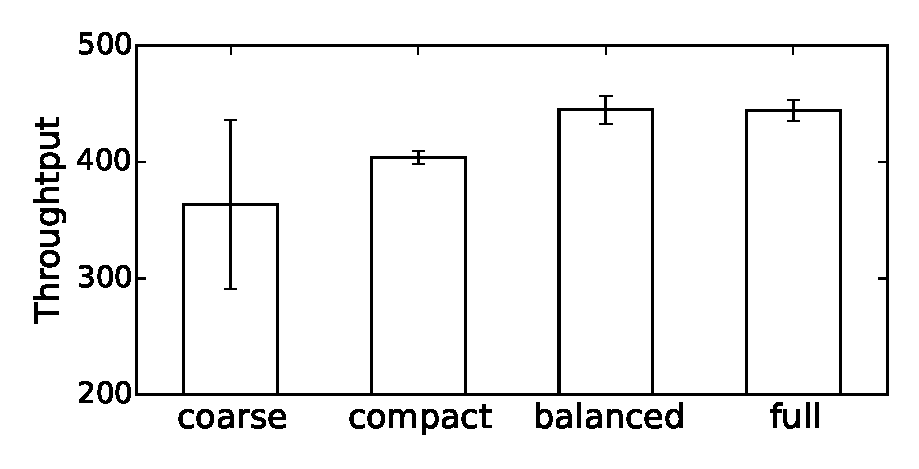
\includegraphics[width=\linewidth]{figures/E38_robustness_std_beta.eps}
    \caption{Beta}
    \label{fig:robustness_beta}
\end{subfigure}
\begin{subfigure}[b]{0.6\textwidth}
    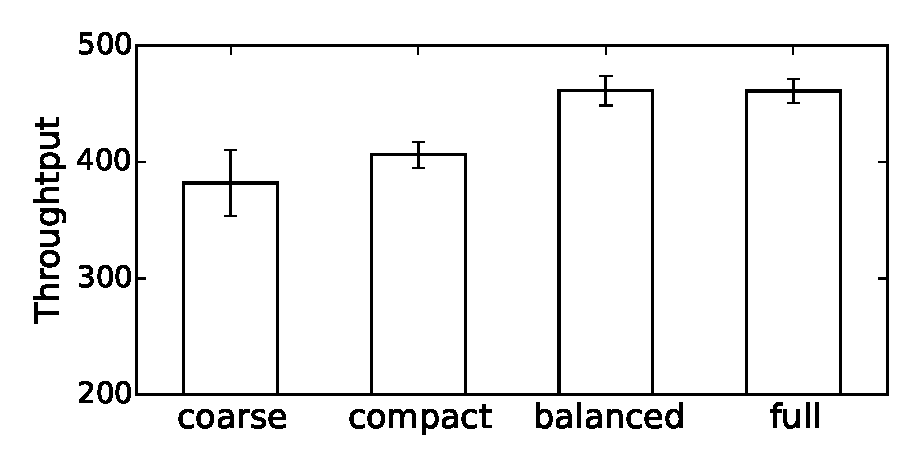
\includegraphics[width=\linewidth]{figures/E38_robustness_std_powerlaw.eps}
    \caption{Power Law}
    \label{fig:robustness_powerlaw}
\end{subfigure}
\begin{subfigure}[b]{0.6\textwidth}
    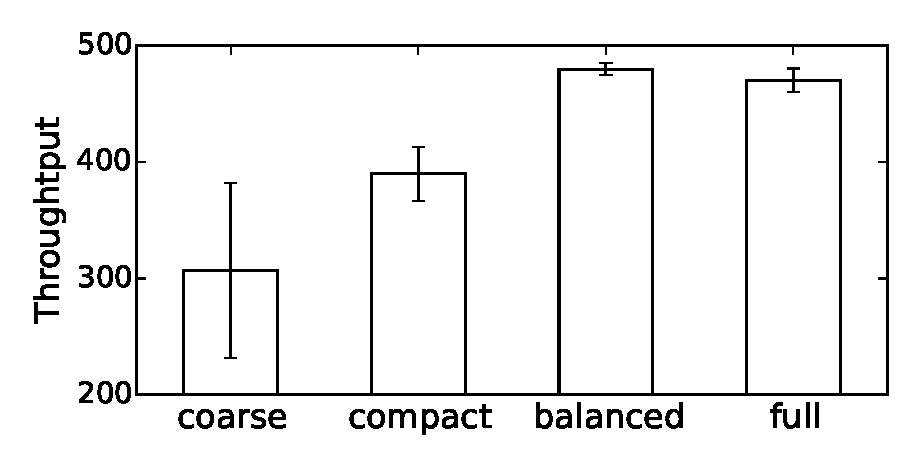
\includegraphics[width=\linewidth]{figures/E38_robustness_std_gamma.eps}
    \caption{Gamma}
    \label{fig:robustness_gamma}
\end{subfigure}
    \centering
    \caption{Compare robustness under slight workload mispredictions. The $y$-axis represents queries per second, and starts from 200 for better presentation to tell performance difference.}
    \label{fig:robustness}
\end{figure}


\subsubsection{Local Storage}

Our evaluation starts with storing data required for Roxie queries
on local disks.
This evaluation involves 8 Roxie nodes: $M=4$ and $R=2$.
\mytable{\ref{tab:throughput_comparison_local}} shows the throughput
of proposed replication and placement schemes under
different workloads.
The values in parenthesis are the speedup relative to \emph{base} performance at
the top of each column.
The \emph{base} placement strategy is uniform.
It does not perform well as
the skewness of workload increases.
For example, the power law workload in the uniform data placement
can only achieve $52.3\%$ of the throughput of a uniform workload.
The second strategy is also coarse grain but replicates according to
anticipated workload.
On a uniform workload this is the same as \emph{base}.
It out performs \emph{base} on skewed workloads.
For example, it
achieves $84.9\%$ more throughput than \emph{base} on \emph{power law}.


Two fine-grain approaches, \emph{compact} and \emph{balanced}, which
further improve performance over \emph{coarse}, are also shown.
In the normal workload case, \emph{compact} and \emph{balanced}
improve on \emph{coarse} by an additional $10.6$ and $78.5$ queries per second.
In the gamma case, \emph{balance} adds $146.2$ queries,
a $47.2\%$ improvement over \emph{coarse}.
Workload-aware data placement is preferable for non-uniform workloads.
The fine-grain strategies out perform \emph{coarse} on all the skewed
workloads.
This is attributed to better load balancing.
As skew increases, the benefit from fine-grain increases (because the
load imbalance in \emph{coarse} increases).


\begin{comment}
\begin{table*}[h]
\centering
\caption{Steady-State Throughput Comparison}
\begin{tabular}{llllll}
\toprule
{} &  Uniform & Beta &  Normal &  Power Law &   Gamma \\
\midrule
Base          & 399.0           &  267.0          &  227.0           &    180.0           &  159.0 \\
Coase         & -               &  368.0 ($38\%$) &  362.0 ($59\%$)  &    371.5 ($106\%$) &  309.5 ($\ \ 95\%$) \\
Monochromatic & 402.5 ($0.9\%$) &  409.0 ($53\%$) &  410.0 ($81\%$)  &    403.5 ($124\%$) &  399.0 ($151\%$) \\
Rainbow       & 426.0 ($6.8\%$) &  431.0 ($61\%$) &  405.5 ($79\%$)  &    442.0 ($146\%$) &  427.0 ($169\%$) \\
Complete      & 438.0 ($9.8\%$) &  414.0 ($55\%$) &  433.0 ($91\%$)  &    449.0 ($149\%$) &  431.0 ($171\%$) \\
\bottomrule
\multicolumn{6}{r}{unit: queries/second} 
\end{tabular}
\label{tab:throughput_comparison}
\end{table*}
\end{comment}


\begin{table}[t]
\centering
\caption{Steady-State Throughput Comparison (NFS)}
\resizebox{\columnwidth}{!}{%
\begin{tabular}{llllll}
\toprule
{} &  Uniform & Beta &  Power Law &  Normal &   Gamma \\
\midrule
\emph{base}       & 446.1            &  383.1            &  220.2             &    393.3             &  176.4 \\
\emph{coarse}     & -                &  396.4 ($3.5\%$)  &  415.3 ($88.6\%$)  &    379.6 ($29.4\%$)  &  327.9 ($85.9\%$) \\
\emph{compact}    & 403.7 ($-9.5\%$) &  416.2 ($8.7\%$)  &  401.3 ($82.3\%$)  &    407.1 ($38.8\%$)  &  407.8 ($131.1\%$) \\
%Rainbow   & 447.3 ($0.3\%$)  &  428.1 ($11.8\%$) &  474.0 ($61.6\%$)  &    469.0 ($113.0\%$) &  481.5 ($172.9\%$) \\
\emph{balanced}   & 447.6 ($0.3\%$)  &  440.8 ($15.1\%$) &  454.0 ($106.2\%$) &    469.7 ($60.1\%$)  &  485.9 ($175.5\%$) \\
%MCMLB     & 447.9 ($0.4\%$)  &  448.8 ($17.2\%$) &  479.8 ($63.6\%$)  &    455.5 ($106.9\%$) &  482.0 ($173.2\%$) \\
\emph{complete}   & 484.2 ($9.0\%$)  &  485.6 ($26.8\%$) &  492.4 ($123.7\%$) &    495.0 ($68.8\%$)  &  490.0 ($177.8\%$) \\
\bottomrule
\multicolumn{6}{r}{unit: queries/second} 
\end{tabular}
}
\label{tab:throughput_comparison_nfs}
\end{table}


The \emph{complete} solution out performs all others, including both fine-grain
solutions.
This is because while the workload was probabilistically generated
over 30,000 requests.
The workload for each small window of requests does not always reflect
the overall workload.
In such cases, \emph{complete} performs better.
However, \emph{complete} is generally not feasible
when dataset is too large to fit into one node.

Overall, workload-aware data placement significantly increases query throughput.
Using fine partition granularity better balances the load.
\emph{Balanced} performs better than \emph{compact}, indicating that
the benefit of a smaller footprint is less than the cost of poorer load
balancing.
The \emph{balanced} scheme is occasionally competitive with \emph{complete}.

\subsubsection{Remote Storage}
Next, we evaluate our proposed schemes against data storing on remote storage.
The Roxie cluster size and the number of benchmark clients remain the same
with the local storage case.
\mytable{\ref{tab:throughput_comparison_nfs}} details the throughput numbers.
This evaluation confirms the general observations seen in the instance
storage test.
However, the throughput is higher using remote storage.
While somewhat counter intuitive, it is not unheard.
This occurs because local storage uses plain commodity disks and the
% not sure the original sentence is grammerly correct
filer uses high-performance disks as well as aggressive caching.
Moreover, the I/O demand does not exceed the capacity of the NFS server.
Therefore, the additional network traffic is not creating a
performance bottleneck.


\subsection{Robustness Comparison}
\label{sec:robustness}

We are interested in how sensitive a placement scheme is to minor
deviations in the anticipated workload.
(Tables~\ref{tab:throughput_comparison_local} and
\ref{tab:throughput_comparison_nfs} show performance degradation for
major deviations.)
We say a placement scheme is more \emph{robust} when the scheme works
well even when the actual workload is slightly different from the
anticipated workload.
We pick different parameters for generating slight workload variance.
For example, we change the shape parameter in the power law distribution.
Therefore, it becomes either less or more skewed.
We create two less and two more skewed workloads for each type.

\myfigure{\ref{fig:robustness}} shows how different placement schemes react
to workload shifts.
The figure shows the average throughput and the standard deviation
 of the placement schemes under the four ``shifted'' workloads
The figure indicates that the coarse-grain scheme
under performs in both average (lower) and deviation (greater)
compared to the fine-grain schemes.

The \emph{compact} scheme is better than \emph{coarse} but its performance is not as
good as the \emph{balanced} scheme.
The \emph{balanced} scheme overall exhibits higher throughput than
\emph{coarse} and \emph{compact}.
More importantly, \emph{balanced} shows consistent standard deviation
in three workloads.
The highest performance degradations in each workload are
$2\%$, $6\%$ and $3\%$
while the \emph{compact} scheme shows
$3\%$, $5\%$ and $14\%$ (increasing as skewness increases) degradation respectively.
% The \emph{balanced} shows $6\%$ performance loss at most.
% balanced
%  - beta: 436.41 vs 444.75
%  - power law: 442.22 vs. 471.82
%  - gamma: 472.98 vs. 487.88
% compact
%  - beta: 396.85 vs. 410.53
%  - power: 388.71 vs. 408.26
%  - gamma: 350.19 vs. 408.02
The above suggests than \emph{balanced} is more robust then
\emph{compact}, which is robust than \emph{coarse}.
There is little difference between \emph{balanced} and \emph{full} in either
average throughput or standard deviation.
This is because there is little difference in the placement of
partitions---that is, the balanced scheme tends to have a high degree of
unique partitions on each node.



\subsection{Micro Benchmark}

We have presented the steady-state throughput in Section~\ref{sec:throughput}.
In this section, we further examine why different placement schemes
lead to large performance difference.

We investigate resource utilization of different placement schemes
for understanding the tradeoff between the \emph{compact} and
\emph{balanced} scheme. 
We collect system statistics
(\textit{dstat}~\cite{dstat} and \textit{cachestat}~\cite{cachestat})
during the entire benchmark runs.
\mytable{\ref{tab:micro_nfs}} presents the system statistics, and
metrics are normalized to the smallest value in each metric group,
except the \emph{max:mean} ratio. 
This normalization better shows the difference between placement schemes.
Except \emph{mean \%CPU}, a system is more efficient when
the metrics listed are small.
These metrics are collected from the benchmark runs under the gamma workload.
Other workloads present very similar trends.

First, we examine CPU utilization across all Roxie nodes.
The average CPU utilization indicates whether Roxie is fully saturated,
and the \emph{max:mean} metric tells whether loads are well balanced
among Roxie nodes.
In the \emph{base} scheme, CPU utilization is the lowest and load imbalance
is the highest, which explains why uniform data placement under performs.
Workload-aware replication eliminates load imbalance while
improving CPU utilization.
Fine-grain partition further reduces load imbalance,
as in the \emph{balanced} scheme.

\begin{table}[ht]
\centering
\caption{Normalized System Statistics of Roxie Servers}
\resizebox{\columnwidth}{!}{%
\begin{tabular}{lllllll}
\toprule
	& Metrics	&	\emph{base}	&	\emph{coarse} & \emph{compact} & \emph{balanced} & \emph{complete} \\
\midrule
\multirow{2}{*}{Load Balancing} & \% CPU (mean)		& \textbf{1.00} (13\%) & 2.29   & 2.37 & 3.11 & 2.97     \\
		                        & \% CPU (max:mean) & 2.01 & 1.34   & 1.23 & 1.1    & 1.14     \\
\midrule
\multirow{3}{*}{Cache Locality} & cache misses (sum)     & 1.13 & 1.24   & \textbf{1.00} (659K) & 1.26 & 1.22     \\
		                        & dirty pages (sum)     & 1.20 & 1.47   & \textbf{1.00} (200K) & 1.52 & 1.29     \\
		                        & cache sizes (max) & 2.11 & 1.51   & \textbf{1.00} (825MB)   & 1.17 & 1.15     \\
\midrule
\multirow{2}{*}{Efficiency}     & I/O wait (mean) & 1.39 & 6.73   & \textbf{1.00} (2.35\%) & 2.48 & 2.55     \\
		                        & TCP connections (mean)   & 2.40 & 1.53   & 1.31 & 1.10 & \textbf{1.00} (1357) \\
%		                        & disk read         & 2.72 & 2.00   & 1.09 & \textbf{1.00} & 3.48    \\
\bottomrule
\end{tabular}
}
\label{tab:micro_nfs}
\end{table}



Second, we examine the benefits of packing multiple replicas into the same node,
as in the \emph{compact} scheme.
\mytable{\ref{tab:micro_nfs}} shows that cache misses and dirty pages
are significantly lower in the \emph{compact} scheme.
Besides, \emph{compact} has much lower cache sizes, $17\%$ lower than
\emph{balanced} and $51\%$ less than the \emph{coarse} scheme.
Although the \emph{compact} scheme outperforms others in cache locality and
requires less cache,
it does not generate the highest query throughput.
A possible explanation is that requests do not greatly benefit from better cache locality.
We suspect the \emph{compact} scheme is useful especially when query applications
require costly read operations.
% We will need to further investigate this case.

Third, we compare I/O wait time and the number of TCP connections
for comparing their efficiency.
A lower I/O wait time indicates that systems do not waste much time on slow I/O operations.
The \emph{compact} scheme, with maximum cache locality, has the lowest I/O wait value.
The number of TCP connections at a given time is related to processing efficiency.
We observe that the \emph{balanced} scheme yields a lower number of TCP connections
than the other schemes, suggesting that requests complete more quickly.


\subsection{Summary}
Our evaluation provides empirical data to support our findings
in the simulation.
First, workload-aware data placement, both the coarse and fine grain methods,
reduces load imbalance, thereby improving system throughput.
However, the coarse-grain approach is insufficient
when workload is highly skewed.
Finer partitioning further balances the loads and in many cases,
the \emph{balanced} scheme has comparable performance to \emph{complete}
(an ``idealistic'' placement).
Furthermore, both \emph{balanced} and \emph{full} are robust while
\emph{compact} reduces storage footprint to $1/R$. 


